\section{必須課題}
\subsection{問題1}
\begin{itemize}
    \item 許容解: 最適化問題において、集合\(S\)の要素\(\bm{x}\)のこと。
    \item 目的関数: 最適化問題において、最大化したい関数\(f(\bm{x})\)のこと。
    \item 最適解: 任意の\(\bm{x} \in S\)に対して\(f(\bm{x}) \geq f(\bm{x}^*)\)となる許容解\(\bm{x}^*\)のこと。
    \item 最適値: 目的関数値の上界の最小値。
\end{itemize}

\subsection{問題2}
\subsubsection{(a)}
\hspace{1em}\((x, y) = (6, -6)\)を条件式の左辺に代入して計算すると

\begin{equation}
    3 \times 6 +2 \times (-2) = 6
\end{equation}

\noindent となり、条件式の右辺の値に一致するため\((6, -6)\)はこの最適化問題の許容解である。

\subsubsection{(b)}
\hspace{1em}\((x, y) = (0, 3)\)とすると、\(0^2 + 3^2 = 9\)で目的関数値をとり、かつ\(3 \times 0 + 2 \times 3 = 6\)で条件も満たすため、これが題意を満たす許容解の1つである。

\subsubsection{(c)}
\hspace{1em}\(x^2 + y^2  = k^2\)とおくと、最適化問題は条件\(3x + 2y = 6\)を満たしたうえで\(k^2\)を最小化するような\(\bm{x}\)を見つける問題になる。 \\
\hspace{1em}さて、\(x^2 + y^2 = k^2\)は\(x-y\)平面上の原点中心で半径が\(k\)の円を表している。
したかって求める\(k\)の値は原点から直線\(3x + 2y = 6\)への距離の値に等しい。
点と距離の直線公式を用いると\(k\)の値は

\begin{align}
    k   &= \frac{|3 \times 0 + 2 \times 0 - 6|}{\sqrt{3^2 + 2^2}} \\
        &= \frac{6}{\sqrt{13}}
\end{align}

\noindent であるから最適値は\(k^2 = \frac{36}{13}\)と求まる。 \\
\hspace{1em}次に最適値を与える最適解を求める。
最適解を求めるには以下の連立方程式を解けば良い。

\begin{equation} 
    \left\{ \,
        \begin{aligned}
            &   x^2 + y^2 = \frac{36}{13} \\
            &   3x + 2y = 6
        \end{aligned}
    \right.
\end{equation}

\noindent 2つ目の式を\(y\)について整理して1つ目の式に代入すると\(x\)は次のように求まる。

\begin{align}
    x^2 + \left(-\frac{3}{2}x + 3\right)^2  &= \frac{36}{13}    \\
    \left(x - \frac{18}{13}\right)^2        &= 0                \\
    x                                       &= \frac{18}{13}
\end{align}

\noindent 次に連立方程式の2式目に得られた\(x\)の値を代入して\(y\)の値を求めると\(y = \frac{12}{13}\)となる。
よって、最適解は\(\left(x, y\right) = \left(\frac{18}{13}, \frac{12}{13}\right)\)となる。

\subsection{問3}
\hspace{1em}(b)がありえない。

\subsection{問4}
\subsubsection{定式化}
\hspace{1em}製品Ⅰを\(x\)単位、製品Ⅱを\(y\)単位生産すると設定すると、最適化問題は以下のように定式化できる。

\begin{equation}
    \left\{ \,
        \begin{aligned}
            & \text{目的関数: } 3x + 2y \\
            & \text{条件1: } 5x + y \leq 10 \\
            & \text{条件2: } x + 2y \leq 5 \\
            & \text{条件3: } x, y \geq 0
        \end{aligned}
    \right.\
\end{equation}

\subsubsection{実行可能領域の図示}
\hspace{1em}以上の定式化をもとにこの最適化問題の実行可能領域を図示すると以下のようになる。

\begin{figure}[H]
    \centering
    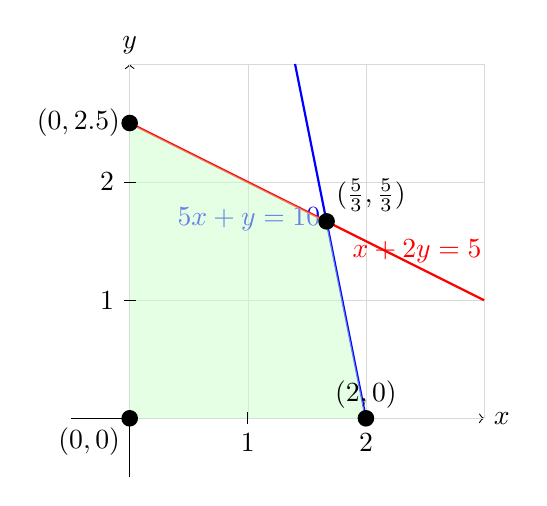
\begin{tikzpicture}[scale=1.5]
        % 軸の描画
        \draw[->] (-0.5,0) -- (3,0) node[right] {$x$};
        \draw[->] (0,-0.5) -- (0,3) node[above] {$y$};
        
        % グリッド
        \draw[help lines, gray!30] (0,0) grid (3,3);
        
        % 制約条件の直線
        % 条件1: 5x + y = 10 → y = 10 - 5x
        \draw[thick, blue] (1.4,3) -- (2,0) node[pos=0.5, above left] {$5x + y = 10$};
        
        % 条件2: x + 2y = 5 → y = (5-x)/2
        \draw[thick, red] (0,2.5) -- (3,1) node[pos=0.6, below right] {$x + 2y = 5$};
        
        % 実行可能領域の塗りつぶし
        \fill[green!20, opacity=0.5] (0,0) -- (0,2.5) -- (1.667,1.667) -- (2,0) -- cycle;
        
        % 頂点の描画
        \fill (0,0) circle (2pt) node[below left] {$(0,0)$};
        \fill (0,2.5) circle (2pt) node[left] {$(0,2.5)$};
        \fill (2,0) circle (2pt) node[above] {$(2,0)$};
        \fill (1.667,1.667) circle (2pt) node[above right] {$(\frac{5}{3},\frac{5}{3})$};
        
        % 座標軸の目盛り
        \foreach \x in {1,2}
            \draw (\x,0.05) -- (\x,-0.05) node[below] {\x};
        \foreach \y in {1,2}
            \draw (0.05,\y) -- (-0.05,\y) node[left] {\y};
    \end{tikzpicture}
    \caption{実行可能領域}
\end{figure}